
\documentclass[10pt]{article} 

\usepackage[utf8]{inputenc} 
\usepackage{geometry} 
\usepackage{pgfplots,wrapfig}
\usepackage{amsmath}
\usepackage{amssymb}
\usepackage{listings}
\usepackage{subcaption}
%\captionsetup[subfigure]{font=scriptsize}
\usepackage{placeins}

 \geometry{
	a4paper,
	total={170mm,257mm},
	left=10mm,
	right=10mm,
	top=20mm,
}

\vspace{2cm}

\setlength{\parindent}{0cm}
\setlength{\parindent}{1em}
\title{A.M.R. Project report}
\author{Caterina Lacerra, Jary Pomponi}
\renewcommand{\lstlistingname}{Algorithm}
\usepackage[colorlinks=true,linkcolor=blue,urlcolor=black,bookmarksopen=true]{hyperref}

\usepackage{bookmark}
\begin{document}
	\maketitle
	\section{Introduction}
	In this project we have studied the problem of motion planning. More precisely we have used and compared different algorithm. 
	
	Informally speaking, the motion planning problem aims to find a path, for a specified robot, from a point A to a point B avoiding obstacles. In practices this problem is very hard for a computational complexity point of view, since need to map the environment in the configuration space of the robot. 
	
	The strength of the algorithm that we have used is that, instead of build and use an explicit representation fo the robot in its configuration space, they rely on a collision checking module. With this approach we build a graph of feasible trajectories in the obstacle free space. The the road map can be used to build the solution for planning problem for a specific robot.
	
	\section{Motion planning problem}
	In this section we will define the planning problem and the primitive procedure that will be used by the algorithms, then we will expose them.
	
	\subsection{Problem formulation}
	In this section we will formalize the problem of path planning.\\
	
	Let $\chi \in(0,1)^d$ be the configuration space, where $d\in\mathbb{N}$ with $d\ge2$, and $\chi_{obs}$ is the obstacle region of the space. The $\chi_{free}$ is the portion of the space that does not contains obstacles.
	The we define an initial position $x_{init} \in \chi_{free}$ and a goal region $\chi_{goal} \subset \chi_{free}$. A path planing problem is defined by a triple $(\chi_{free},x_{init},\chi_{goal}) $. 
	
	The goal of a path planner is to find a feasible path from $x_{init}$ to $\chi_{goal}$ in $\chi_{free}$, if exists, and report failure otherwise.\\
	
	To do this we build a DAG (direct acyclic graph) of possible road maps from the initial point to the other point in $\chi_{free}$. The we get the optimal path from all the possible ones.
	
	\subsection{Primitive procedures}
	Before discussing the implemented algorithm we introduce the principal procedures that we will use.\\
	
	\textbf{SampleFree:} is a function that return a point $x_{r} \in \chi_{free}$. The samples are assumed to be draw from a uniform distribution, and each one is independent from others.\\
	
	
	\textbf{NearestNode:} Given a a graph $G=(V,E)$ and a point $x\in\chi_{free}$, where $v\subset\chi$, the function return a point $x_{near} \in V$ that is the closest to $x$ given the euclidean distance. Formally: 
	\begin{align}
    getNearest (G,x) := argmin_{v \in V} ||x - v|| \nonumber
	\end{align}
	The are other two versions of the method. One version of this function, taken another value r, will return a set of $x\in V$ that are contained in a ball of radius $r$ centred in $x$, the other one return k nearest vertex to $x$.\\  
	
	\textbf{Steer:} Given two point $x,y \in \chi$, the function steer returns a point $z \in \chi$ that minimize the distance from $z$ to $y$ while $||z-x|| \le \eta$, with $\eta > 0$. \\
	
	\textbf{collisionFree:} Given two point $x,y \in \chi_{free}$ the function return true if the line that connect $x$ to $y$ lies in $\chi_{free}$.\\
	
	\textbf{Parent:} Given a Graph $G=(V,E)$ and an $x\in V$, the method return a point $y \in V$ that satisfy $(y,x) \in E$. By convention, if $x$ is the root node of $V$ this function will return $x$.\\
	
	\textbf{Line:} Given two points $x,y \in \chi$, the methods return a line that go from the point $x$ to the point $y$.\\
	
	\textbf{Cost:} Given a graph $G=(V,E)$, a node $v_{start} \in V$ and another node $v_{goal} \in V$, the methods will return the cost $c \in\mathbb{R}$ of the unique path from $v_{start}$ to the node $v$. By convention the cost of the root node is zero. If only one node is give, the method return the distance from the root of the graph to $v_{goal}$.\\

	\subsection{Existing Algorithm}

	Rapidly-exploring Random Trees (RRT) based algorithm are very effective for solving the path planning problem for high complex configuration space. This because that class of algorithm combine random sampling of the configuration space with biased sampling around a desired goal. A good property that follow from the random sampling is that the construction of the tree growth is biased towards unexplored areas of the configuration space.
	
	This class of algorithm aim to build a road-map graph in the configuration space from a root tree to a feasible goal region. Another property of this class is that the algorithms are single query, so each road-map is relative to a single problem. 
	
	While RRTs have been show to be extremely effective at generating feasible solution in the configuration space, they provide no control on the quality of the found path. This problem is accentuated if the space contains non uniform cost sub-spaces. And for a robot in a real world is important to find a good path in a fast way.
	
	The basic behaviour of this class of algorithms are the following one: at each iteration the algorithm  sample a new point in the free space. Then calculate the nearest vertex in V to the sampled point, and then the algorithm tries to connect the nearest vertex to this random point, using the \textbf{Steer} function. If the connection does not collide with any obstacles, the new vertex and the edge, that connects the new point and the nearest one, are added to the graph. This is show in \textit{figure 1}.
	
		
	The algorithms in this section are probabilistic complete. This means that, if a path exist from the initial vertex to the goal one, the probability that the algorithm fails to find that path asymptotically approaches zero with $n \rightarrow \inf$. 
	
	
	\FloatBarrier
	\begin{figure}[bht]
		\centering
		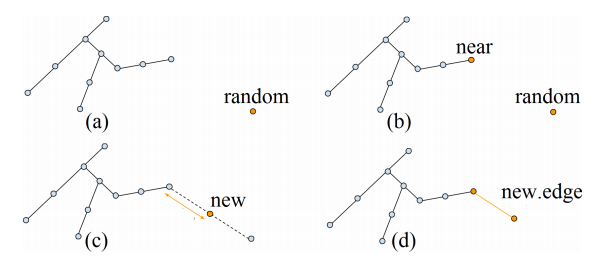
\includegraphics[width=0.8\linewidth]{rrtExt.png}
		\caption{The extending procedure}
	\end{figure}
\FloatBarrier
	\subsubsection{Rapidly-exploring Random Trees (RRT)}
	
	This is the simplest RRT algorithm. In this basic version, the algorithm does not take into account the distance of the path, if one is found, from the start vertex to the goal region. On the other it is very fast in exploring, randomly, the configuration space.

	In this version of the algorithm we perform the basic operations n times, so the algorithm does not stop if reach the goal but keep running until the number of iteration is not reached. 
	\begin{lstlisting}[frame=single, mathescape=true,caption={RRT}]
G = ($x_{init},\emptyset$)
for i = 1$\dots$ n do
	$x_{rand} \leftarrow$ SampleFree
	$x_{nearest}  \leftarrow$ NearestNode(G,$x_{rand}$)
	$x_{new} \leftarrow Steer(x_{nearest},x_{rand})$	
	if collisionFree($x_{nearest},x_{new}$) then
		$V \leftarrow V \cup \{x_{new}\}$
		$E \leftarrow E \cup \{
		(x_{nearest}
		,x_{new}
		)\}$
	\end{lstlisting}
	
	One negative results tell us that the cost of the best path found by the RRT procedure converges to a random variable. This implies that the cost of the solution converges to a suboptimal value, with probability one. It is possible to implements different heuristic in order to improve the solution, but the the sub-optimality still. So this basic algorithm is probabilistic complete but not asymptotic optimal.
	
	\subsubsection{Anytime RRT}
	
	The main idea behind this approach is that we have a limited amount of time. In this time we run a basic RRT algorithm, and if there is some time left, it tries to generate a new RRT path ensuring that the cost of than new path is lower than the previously found. This is achieved by limiting the nodes added to the tree to the only ones that can contribute to a solution with lower overall cost. 
	
	This approach assures that each new tree contains a path that cost less regard all the previously trees. However this approach does not guarantees that a new solution can be produced. To ensure that the new solution will cost less then the previously one the algorithm incorporate cost consideration and bias factor on the methods.
	
	\noindent\begin{minipage}{.48\textwidth}
		\begin{lstlisting}[frame=single, mathescape=true,caption={Anytime RRT}]
$\textbf{Main}$()
 $G = (x_{start}, \emptyset)$
 $d_{b} \leftarrow 1$
 $c_{b} \leftarrow 0 $
 $c_{s} \leftarrow \inf$
 loop
  $G = (x_{start}, \emptyset)$
  $c_{n} \leftarrow \textbf{growRRT}(G)$
  if($c_{n} \ne \textbf{null}$) then
   $\textbf{postCurrentSolution}(G)$
   $c_{s} \leftarrow (1 -\epsilon)*c_{n}$
   $d_{b} \leftarrow d_{b} - \delta_{d}$
   if ($db_{<0} $) then
   	$d_{b} \leftarrow 0$
   $c_{b} = c_{b} + \delta_{d}$
   if ($c_{b}>1$) then
   	$c_{b} \leftarrow 1$
$\textbf{chooseTarget}$(G)
 $rand \leftarrow randomRealIn [0,1]$
 if (rand > goalBias)
  return $x_{goal}$
 else
  $x_{new} \leftarrow RandomFreeConfig()$
  attemp $\leftarrow 0$
  while ($cost(x_{start},x_{new})$
     + $cost(x_{new},x_{goal}) > c_{s}$ ) do
   $q_{new} \leftarrow RandomFreeConfig()$
   attemp $\leftarrow$ attemp+1
   if(attemp > maxAttemp) then
    return null
  return q_{new}
   
 		\end{lstlisting}
\end{minipage}
\hfil
\noindent\begin{minipage}{.48\textwidth}
		\begin{lstlisting}[frame=single,basicstyle=\small, mathescape=true,caption={Anytime RRT}]
$\textbf{GrowRRT}$()
 $x_{new} \leftarrow x_{start}$
 $time \leftarrow 0$
 while($||x_{new}-x_{goal}||$> Threshold) do
  $x_{target} \leftarrow \textbf{chooseTarget}(G,x_{target})$
  if ($x_{target} \ne null$) then
   $x_{new} \leftarrow \textbf{extendToTarget}(G,x_{target})$
   if$( x_{new} \ne null )$ then
    $V \leftarrow V \cup \{x_{new}\}$
    $\textbf{updateTime}(time)$
    if (time > maxTimePerRRT) then
     return null
  return \textbf{distance}($x_{start}, x_{new}$)
$\textbf{extendToTarget}$(G,$x_{target}$)
 $K_{near} \leftarrow \textbf{kNearestNeighbors}(G,x_{target},k) $ 
 while $K_{near}$ is no empty do
  remove $x_{tree}$ with minimum 
    $selCost(G,x_{tree},x_{target})$ from $K_{near}$
  $Q_{ext} \leftarrow \textbf{generalExtensions}(x_{tree},x_{target})$
  $x_{new} \leftarrow \textbf{argmin}_{q \in Q_{ext}} ||x_{tree} -x ||$
  $c \leftarrow \textbf{cost}(x_{start},x_{tree}) +
    ||x_{tree} - x_{new} ||$
  if $c + \textbf{cost}(x_{new},x_{goal}) < c_{s}$ then
   return $x_{new}$
 return null
$\textbf{SelCost}(G,x,x_{target})$
 return $d_{b}*\textbf{distance}(x,x_{target}) + $
   $c_{b} * \textbf{cost}(x_{start},x)$
\end{lstlisting}
\end{minipage}


	\subsubsection{RRT*}
	
	This algorithm still use a tree graph, but with the improvement that the graph are modified at each iteration, if it discover better path from the root to the actual node.
	
	This algorithm add a point to the graph in the same way as RTT does, but it also consider connection from a subset of the vertex called xNear. This set contains the nodes that are inside a ball of radius 
	\begin{align}
		 min\left\{\gamma_{RRT}\left(\frac{log(card(V)}{card(V)}\right)^{1/d},\eta\right\}
		\nonumber
	\end{align}
	
	where d are the dimension of the configuration space $\chi$, $\eta$ is the constant of steering function and $\gamma_{RRT}$ are a constant related related to the shape of the configuration space, and it is equal to
	
	\begin{align}
	2\left(1+\frac{1}{d}\right)^{1/d} \left(\frac{\mu(\chi_{free})}{\varsigma_{d}}\right)^{1/d}
	\nonumber
	\end{align}
	
	where  $\mu(\chi_{free})$ denotes the volume of the free space and $\varsigma_{d}$ is the volume of the unit ball in the d-dimensional 	Euclidean space.
	
	In our case d is equal to 2.
	
		\begin{lstlisting}[frame=single, mathescape=true,caption={RRT*}]
G = ($x_{init},\emptyset$)
for i = 1$\dots$ n do
 $x_{rand} \leftarrow \textbf{SampleFree}$
 $x_{nearest}  \leftarrow \textbf{NearestNode}(G,x_{rand}$)
 $x_{new} \leftarrow \textbf{Steer}(x_{nearest},x_{rand})$	
   if $\textbf{collisionFree}$($x_{nearest},x_{new}$) then
	$radius \leftarrow min\{\gamma_{RRT}(\frac{log(card(V)}{card(V)})^{1/d},\eta\}$
	$xNear \leftarrow \textbf{nearestNode}(G,x_{new},radius)$
	$V \leftarrow V \cup \{x_{new}\}$
	$x_{min} \leftarrow x_{nearest}$
	$c_{min} \leftarrow \textbf{Cost}(x_{nearest}) + ||x_{nearest} - x_{new} ||$
	foreach $x_{near} \in xNear$ do
	   if $\textbf{collisionFree}(x_{near}, x_{new} ) \wedge \textbf{Cost}(x_{near}) + ||x_{near} - x_{new} || < c_{min}$
	   then
	        $x{min} \leftarrow x_{near}$
		$c_{min} \leftarrow \textbf{Cost}(x_{near}) + ||x_{near} - x_{new} ||$
	$E \leftarrow E \cup \{
	(x_{min}
	,x_{new})\}$
	foreach $x_{near} \in xNear$ do
	   if $\textbf{collisionFree}(x_{near}, x_{new} ) \wedge Cost(x_{near}) + ||x_{near} - x_{new} || < \textbf{Cost}(x_{near})$
	   then
	     $x_{parent}\leftarrow \textbf{Parent}(x_{near})$
	     $E \leftarrow (E \diagdown \{(x_{parent},x_{near})\} \cup \{(x_{new},x_{near})\})$
	
	\end{lstlisting}
	\FloatBarrier
	\begin{figure}
		\centering
		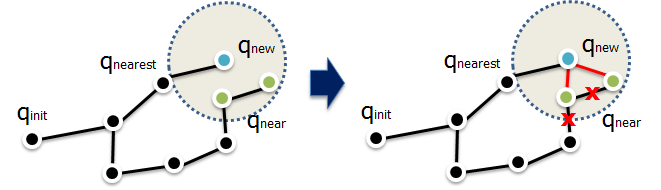
\includegraphics[width=\linewidth]{rrtRew.png}
		\caption{The rewrite process}
	\end{figure}
	\FloatBarrier
	The basic iteration are the same of RRT. The main difference is that, if the connection between $x_{nearest}$ and $x_{new}$ is collision free, the algorithm get all the configuration inside the ball centred in $x_{new}$. Then, we get the configuration in the sphere that minimize the the cost of the path from $x_{init}$ to that configuration, passing trough $x_{new}$, and connect that configuration to $x_{new}$.
	
	After that the algorithm rewrite the tree. For each configuration inside the sphere the algorithm check if is convenient to change the father of that configuration with $x_{new}$. This is true if the cost of the path will be lower passing trough $x_{new}$.
	
	The rewrite process is show in \textit{figure 2}.

	
	\section{Set up and Experiments}
	In this section we will explain the implementation and we'll show the results of the experiments.
	\subsection{Implementation of the algorithm}
	\subsection{Experiments}
	
	
\begin{figure}
	\begin{subfigure}{\textwidth}
		\centering
		\begin{minipage}[b]{0.32\linewidth}
		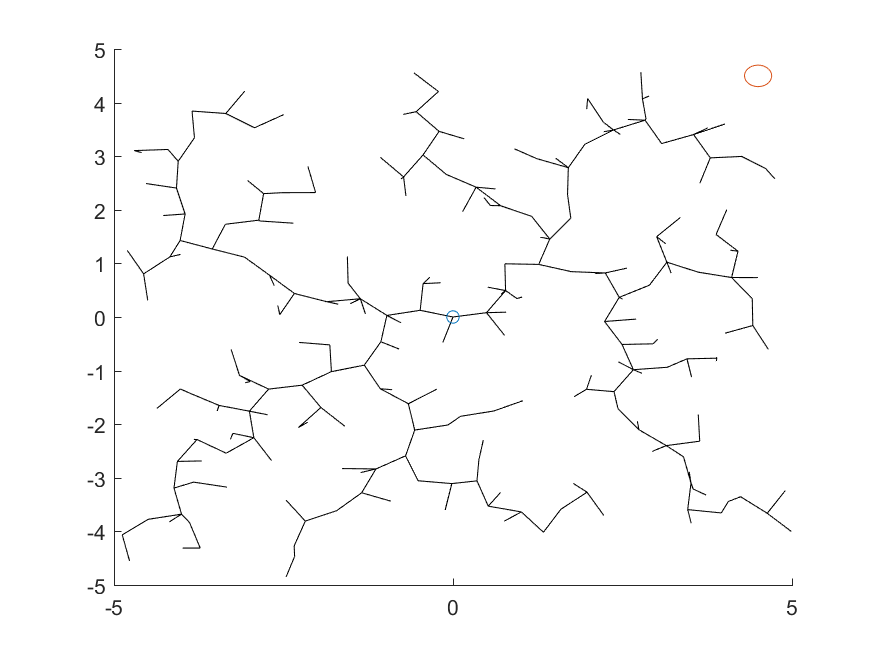
\includegraphics[width=\linewidth]{empty_250_dist_0}
		\caption{RRT after 250 iterations}
	\end{minipage}
		\begin{minipage}[b]{0.32\linewidth}
		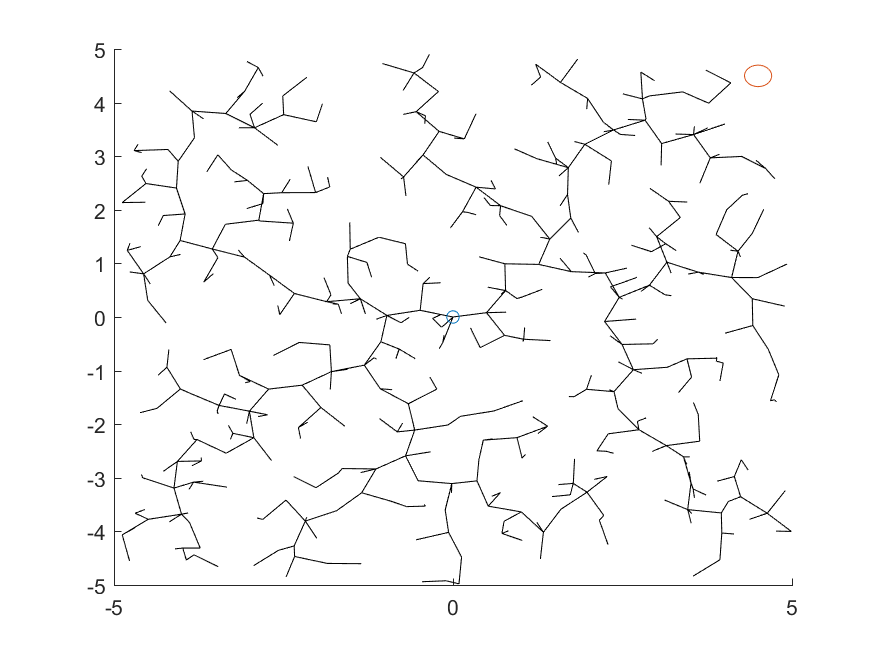
\includegraphics[width=\linewidth]{empty_500_dist_0}
		\caption{RRT after 500 iterations}
	\end{minipage}
		\begin{minipage}[b]{0.32\linewidth}
		\includegraphics[width=\linewidth]{{empty_2500_dist_7.915}.png}
		\caption{RRT after 2500 iterations}	
	\end{minipage}
\end{subfigure}
	\begin{subfigure}{\textwidth}
		\centering
		\begin{minipage}[b]{0.32\linewidth}
			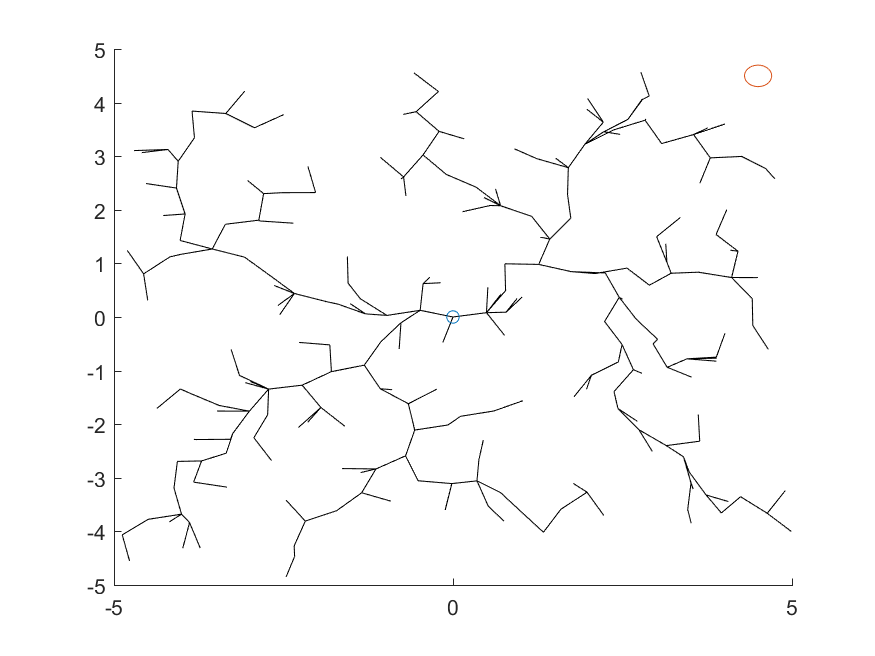
\includegraphics[width=\linewidth]{rrts_empty_250_dist_0}
			\caption{RRT* after 250 iterations}
		\end{minipage}
	\hfill
		\begin{minipage}[b]{0.32\linewidth}
			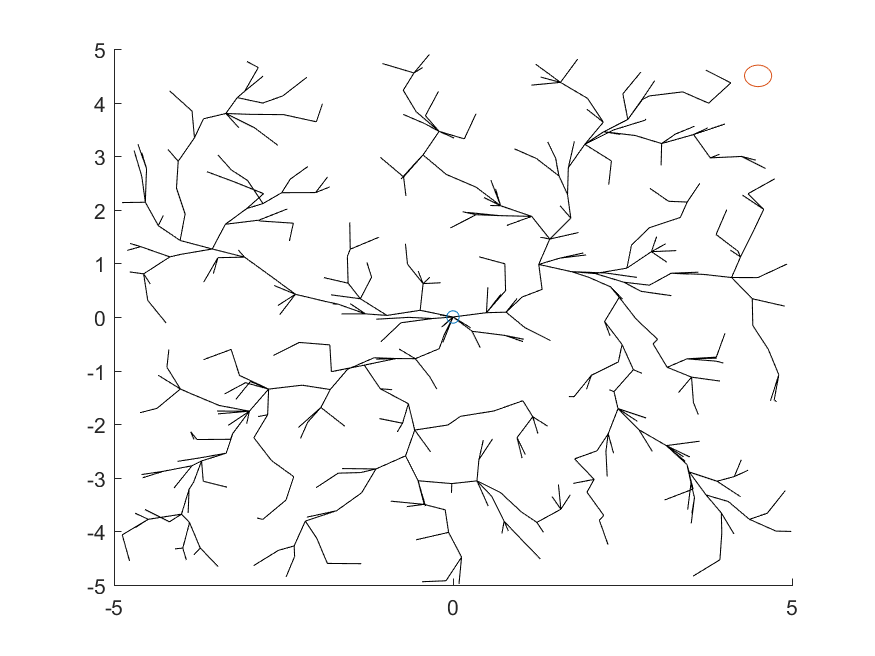
\includegraphics[width=\linewidth]{rtts_empty_500_dist_0}
			\caption{RRT* after 500 iterations}
		\end{minipage}
	\hfill
		\begin{minipage}[b]{0.32\linewidth}
			\includegraphics[width=\linewidth]{{rtts_empty_2500_dist_6.6714}.png}
			\caption{RRT* after 2500 iterations}	
		\end{minipage}
	\end{subfigure}
	\begin{subfigure}{\textwidth}
		\centering
			\begin{minipage}[b]{0.45\linewidth}
				\includegraphics[width=\linewidth]{{empty_5000_dist_7.915}.png}
				\caption{RRT after 5000 iterations}
			\end{minipage}
		\hfill
			\begin{minipage}[b]{0.45\linewidth}
				\includegraphics[width=\linewidth]{{rtts_empty_5000_dist_6.4041}.png}
				\caption{RRTS* after 5000 iterations}
			\end{minipage}
	\end{subfigure}
\caption{The configuration exploration differences between RRT and RRT* in an empty space, without goal bias.}
\end{figure}


\begin{figure}
	\begin{subfigure}{\textwidth}
		\centering
		\begin{minipage}[b]{0.32\linewidth}
			\includegraphics[width=\linewidth]{{OBJ_RRT_5000_dist_6.3905}.png}
			\caption{RRT}
		\end{minipage}
	\hfill
		\begin{minipage}[b]{0.32\linewidth}
			\includegraphics[width=\linewidth]{{OBJ_RRTS_5000_dist_6.1611}.png}
			\caption{RRT*}
		\end{minipage}
	\hfill
		\begin{minipage}[b]{0.32\linewidth}
			\includegraphics[width=\linewidth]{{rtts_empty_2500_dist_6.6714}.png}
			\caption{Anytime RRT}	
		\end{minipage}
	\end{subfigure}
	\begin{subfigure}{\textwidth}
		\centering
		\begin{minipage}[b]{0.32\linewidth}
			\includegraphics[width=\linewidth]{{OBJ_2_RRT_5000_dist_21.0447}.png}
			\caption{RRT}
		\end{minipage}
		\hfill
		\begin{minipage}[b]{0.32\linewidth}
			\includegraphics[width=\linewidth]{{OBJ_2_RRTS_5000_dist_15.0202}.png}
			\caption{RRT*}
		\end{minipage}
		\hfill
		\begin{minipage}[b]{0.32\linewidth}
			\includegraphics[width=\linewidth]{{rtts_empty_2500_dist_6.6714}.png}
			\caption{Anytime RRT}	
		\end{minipage}
	\end{subfigure}
	\begin{subfigure}{\textwidth}
		\centering
		\begin{minipage}[b]{0.32\linewidth}
			\includegraphics[width=\linewidth]{{OBJ_1_RRT_5000_dist_13.7746}.png}
			\caption{RRT}
		\end{minipage}
		\hfill
		\begin{minipage}[b]{0.32\linewidth}
			\includegraphics[width=\linewidth]{{OBJ_1_RRTS_5000_dist_11.1521}.png}
			\caption{RRT*}
		\end{minipage}
			\hfill
	\begin{minipage}[b]{0.32\linewidth}
		\includegraphics[width=\linewidth]{{rtts_empty_2500_dist_6.6714}.png}
		\caption{Anytime RRT}
	\end{minipage}
	\end{subfigure}
	\begin{subfigure}{\textwidth}
	\centering
	\begin{minipage}[b]{0.32\linewidth}
		\includegraphics[width=\linewidth]{{OBJ_3_RRT_5000_dist_17.4342}.png}
		\caption{RRT}
	\end{minipage}
	\hfill
	\begin{minipage}[b]{0.32\linewidth}
		\includegraphics[width=\linewidth]{{OBJ_3_RRTS_5000_dist_12.2502}.png}
		\caption{RRT*}
	\end{minipage}
	\hfill
	\begin{minipage}[b]{0.32\linewidth}
		\includegraphics[width=\linewidth]{{rtts_empty_2500_dist_6.6714}.png}
		\caption{Anytime RRT}
	\end{minipage}


	\end{subfigure}
	\caption{Some tests done in different obstacle environment}
\end{figure}

\begin{figure}
	\begin{subfigure}{\textwidth}
		\centering	

		\begin{minipage}[b]{0.45\linewidth}
			\includegraphics[width=\linewidth]{{corridoio_RTTS_5000_dist_6.339}.png}
			\caption{Anytime RRT}
		\end{minipage}
		\hfill
		\begin{minipage}[b]{0.45\linewidth}
			\includegraphics[width=\linewidth]{{rtts_empty_2500_dist_6.6714}.png}
			\caption{RRT*}	
		\end{minipage}
	\end{subfigure}
	\caption{Results in an environment contains non uniforms cost area}
	
\end{figure}
\FloatBarrier
	\section{Conclusion}
\end{document}

